\section{Scenarios as message sequence charts\label{section:background-scenarios}}

Labeled transition systems may capture the behaviors of a single agent class. Scenarios illustrate admissible interactions among multiple agent instances. The scenarios we use in this thesis are specified in a syntactic subset of Message Sequence Charts (MSC)~\cite{ITU:1996}, see Fig.~\ref{image:train-scenario-all-agents} for example. To keep scenario specifications the models usable by end-users, we will use only a small subset of their features. In its simplest form, a MSC is composed of vertical lines representing timelines associated with agent instances and horizontal arrows representing interactions events among them. According to the previous section, events are synchronously sent and received by interacting agents (we will also use the terms \emph{controlled} and \emph{monitored} events, respectively). As already stated in previous section, we assume that an event label uniquely determines the latter agents. 

We consider \emph{positive} scenarios, that are examples of behaviors that the system should exhibit (see Section~\ref{subsection:background-positive-scenarios}), and \emph{negative} scenarios that behaviors that the system must avoid (see Section~\ref{subsection:background-negative-scenarios}). Sections~\ref{subsection:background-scenario-collections}, \ref{subsection:background-hmsc} and \ref{subsection:background-scenario-annotations} will then discuss ways of managing multiple positive and negative scenarios. 

\subsection{Positive scenarios\label{subsection:background-positive-scenarios}}

As in~\cite{Uchitel:2004}, MSCs are given a trace semantics. We will consider that a MSC defines a set of traces; the latter are expressed through a LTS. Given a MSC, two kinds of traces can be considered: those from the local perspective of a single timeline and those from the global perspective of the complete MSC. We discuss each of these views in turn.

As time in a MSC evolves from top to bottom, the order in which events are sent and received along a particular timeline defines a total order. Therefore, from the perspective of a single agent, a MSC defines one simple trace; such trace is \emph{maximal} trace in that it includes all events in which the agent participates. This trace and all its suffixes can be captured by a LTS. For example, the traces defined by the timeline of the \artifact{Controller} in the MSC of Fig.~\ref{image:train-scenario-all-agents} are precisely captured by the LTS in Fig.~\ref{image:local-traces-lts}. Given a MSC $M$ and an agent $Ag$, we will denote such LTS by $M_{\downarrow Ag}$.

\vspace{0.5cm}
\begin{figure}[H]\centering
\scalebox{0.45}{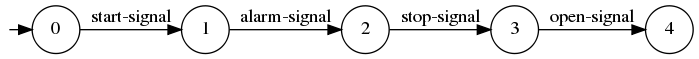
\includegraphics{src/2-framework/images/local-trace}}
\caption{LTS capturing the traces of the MSC in Fig.~\ref{image:train-scenario-all-agents} from the local point of view of the \artifact{Controller}.\label{image:local-traces-lts}}
\end{figure}

When looking at traces from the perspective of the whole MSC, two possibilities might be envisaged.

\noindent \textbf{Total event ordering} -- one might consider that a MSC defines a simple \emph{maximal} trace where all events appear according to the graphical top-down ordering. In our example, such trace would be

\begin{center}\artifact{<start-signal, start, alarm-pressed, \ldots, open>}\end{center} 

A MSC would then define a total order among all events. This leads to a simple and straightforward, yet limited, trace semantics for MSCs.

\noindent \textbf{Partial event ordering} -- when considering concurrent systems, a partial ordering among events seems more adequate~\cite{ITU:1996, Uchitel:2003}. Consider for example the events \artifact{start-signal} and \artifact{alarm-pressed} at the beginning of the MSC shown in Fig.~\ref{image:train-scenario-all-agents}. These two events capture unrelated message passing between different agents; they can therefore hardly be considered ordered over time -- e.g. the passenger might push the alarm button when the \artifact{start-signal} is already sent but before \artifact{start} has been propagated; or maybe even before \artifact{start-signal}; and so on. 

To account for such situations, one has to consider that the traces defined by a MSC are \emph{linearizations} of the partial order among MSC events. In other words, linearizations capture all possible sequences of events that respect the total ordering defined by the timelines. We do not formalize the structure of Message Sequence Charts and their linearizations here, and refer the reader to~\cite{Uchitel:2003} for such a mathematical characterization. 

The set of traces obtained from the local and global perspectives discussed are related ass follows:

\vspace{-0.5cm}
\begin{align}
\mathcal{L}_{total}(M) & \subseteq \mathcal{L}_{partial}(M) \\
\mathcal{L}_{partial}(M) &= \mathcal{L}(M_{\downarrow Ag_1} \parallel \ldots \parallel M_{\downarrow Ag_n})
\label{equation:msc-composition}
\end{align}

The first equation states that the set of traces under a partial ordering includes those under a total ordering. Clearly, the model with partial ordering is more general than the one with total ordering. This means that everything that is true for the former is certainly true for the latter as well. Unless stated otherwise, we will therefore assume the general framework with partial ordering. In particular, we will no longer make the $partial$ and $total$ subscripting explicit when stating other language relations in the following sections.

The second equation above provides a simple way of computing all linearizations of a MSC as an acyclic transition system through LTS composition. Such a LTS is illustrated in Fig.~\ref{image:msc-linearizations} for the MSC in Fig.\ref{image:train-scenario-all-agents}. As shown there, the latter accepts six different linearizations due to the possible interleavings of its first four events. By construction, such a LTS has only one initial state (the leftmost one) and only one terminating state (the rightmost one). This allows us to loosely refer to \emph{the} terminating state of a MSC with a precise underlying meaning; it refers to the LTS capturing its traces.

\aside{The reader wondering whether certain linearizations are \emph{implied} scenarios~\cite{Uchitel:2004} or whether our initial scenario should not be regarded flawed is referred to Section~\ref{section:background-discussion}; those issues are further examined there.}

\begin{figure}\centering
\scalebox{0.31}{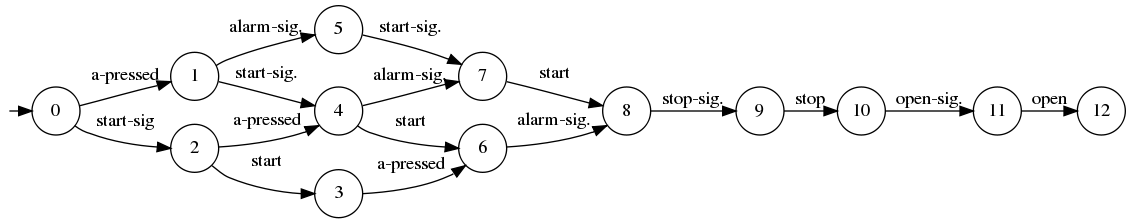
\includegraphics{src/2-framework/images/linearizations}}
\caption{LTS capturing all event linearizations of the MSC in Fig.~\ref{image:train-scenario-all-agents}. Here, \artifact{alarm-pressed} is abbreviated as \artifact{a-pressed} and \artifact{sig.} stands for \artifact{signal}. \label{image:msc-linearizations}}
\end{figure}

\subsection{Negative scenarios\label{subsection:background-negative-scenarios}}

Positive MSCs capture examples of behavior that the system is expected to exhibit. In addition, it is often convenient to specify examples of behavior that the system may \emph{not} exhibit. Proscribed behaviors are illustrated through negative MSCs~\cite{Uchitel:2004}. A negative MSC is a scenario whose last event is prohibited, as depicted by a crossed arrow below a dashed line. Fig.~\ref{image:train-negative-scenario} shows a negative scenario where the \artifact{Controller} may not open doors immediately after having started the train.

\begin{figure}\centering
\scalebox{0.75}{
  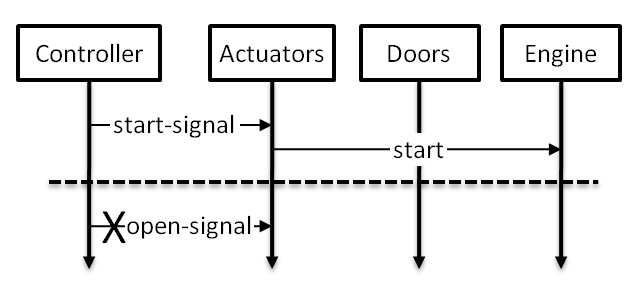
\includegraphics[trim=2mm 2mm 2mm 2mm, clip]{src/2-framework/images/train-negative-scenario}
}
\caption{A negative scenario illustrating that the controller may not open doors after having started.\label{image:train-negative-scenario}}
\end{figure}

More precisely, a negative MSC is a pair $(P,e)$ where $P$ is a positive MSC and $e$ is a single event label. The positive scenario prefix $P$ is called the $precondition$ and $e$ the \emph{prohibited event}. The intuitive semantics is that, once the precondition has occurred from the system's initial state, $e$ may not be the very \emph{next} event in the system. 

We make this semantics fully precise now. First, the precondition of a negative MSC $N = (P,e)$ is a positive MSC; it therefore defines a set of positive traces $\mathcal{L}^{+}$ (as in previous section, we consider the general framework with partial ordering here):

\vspace{-0.2cm}
\begin{equation*}
\mathcal{L}^{+}(N) = \mathcal{L}(P)
\end{equation*}

\noindent In addition, a MSC defines a set of negative traces $\mathcal{L}^{-}$:

\vspace{-0.2cm}
\begin{equation*}
\mathcal{L}^{-}(N) = \{~w.l \mid w \in mt(\mathcal{L}(P)) \wedge l = label(e)~\}
\end{equation*}

\noindent where, for recall, $mt(\mathcal{L})$ denotes the set of maximal traces of the language $\mathcal{L}$ (see Section~\ref{section:background-lts-and-regular-languages}).

That is, negative traces are maximal traces of the precondition concatenated with the label of the proscribed event. Note that the precondition must occur completely for the prohibited event to be taken into account. In other words, partial orderings between the prohibited event and those in the precondition are not considered. This is the intended meaning of the dashed line separating them~\cite{Uchitel:2004}. 

Note that the set of negative traces cannot be captured through a LTS only. This is because $\mathcal{L}^{-}(N)$ is not prefix-closed (see Section~\ref{section:background-lts-and-regular-languages}). Negative scenarios are sometimes captured by a LTS extended with an error state~\cite{Uchitel:2004}. Alternatively, we may use a standard automaton making a distinction between accepting and non-accepting states. 

\subsection{Scenario collections\label{subsection:background-scenario-collections}}

Systems are generally illustrated through multiple positive and negative scenarios. We will therefore consider scenario collections $Sc = (S^+,S^-)$ where $S^+$ and $S^-$ are finite, possibly empty, sets of positive MSCs and negative MSCs, respectively.

The positive and negative languages captured by a scenario collection $Sc = (S^+,S^-)$ are defined via the union operation on languages, taking into account the fact that negative scenarios define positive traces in addition to negative ones:

\vspace{-0.5cm}
\begin{align*}
\mathcal{L}^+(Sc) &= \bigcup_{P \in S^+} \mathcal{L}(P)~~\cup~~\bigcup_{N \in S^{-}} \mathcal{L}^{+}(N) \\
\mathcal{L}^-(Sc) &= \bigcup_{N \in S^-} \mathcal{L}^{-}(N)
\end{align*}

\subsection{Flowcharting scenarios in high-level message sequence charts\label{subsection:background-hmsc}}

A High Level Message Sequence Chart is a directed graph where each node refers to a MSC or a finer grained hMSC~\cite{ITU:1996}. Refered MSCs are called \emph{basic} MSCs, bMSCs for short. Outgoing edges from a node capture possible continuations, allowing the user to introduce sequences, alternatives and loops; to reuse small MSC fragments; and so on. A hMSC has an initial starting point that indicates the initial system state. Fig.~\ref{image:train-hmsc} shows a hMSC for our running example.

\vspace{0.4cm}
\begin{figure}[H]\centering
\scalebox{0.66}{
  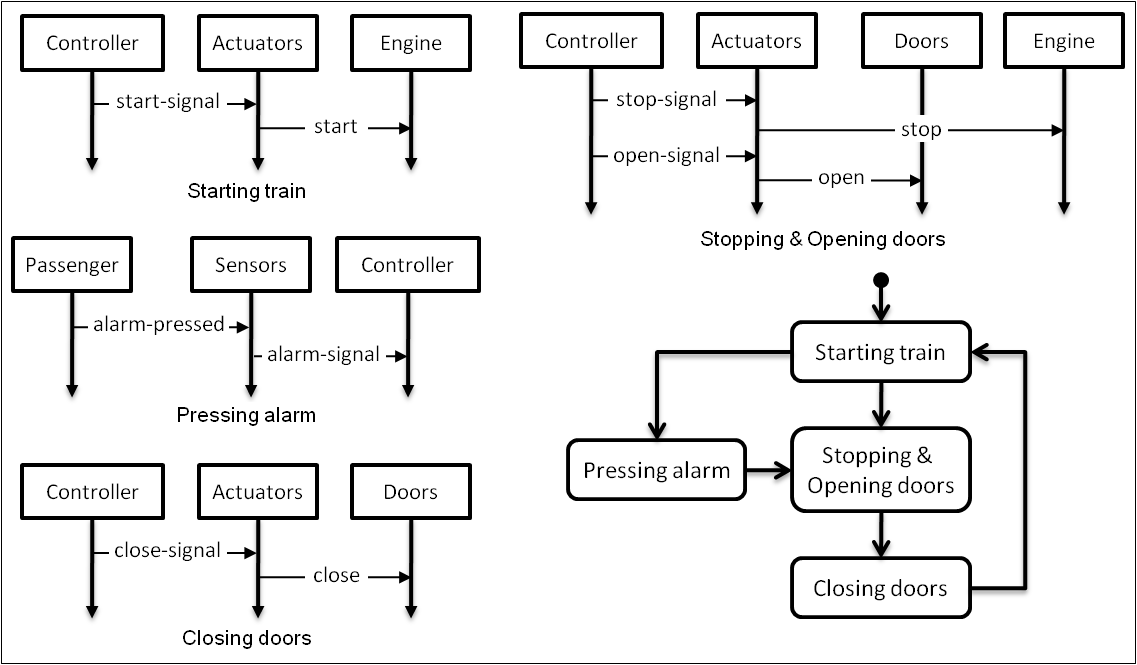
\includegraphics[trim=2mm 2mm 2mm 2mm, clip]{src/2-framework/images/train-hmsc}
}
\caption{A high-level Message Sequence Chart for the train system.\label{image:train-hmsc}}
\end{figure}

The following section provides the trace semantics for hMSCs containing bMSCs only. The semantics is further extended to take finer-grained hMSCs into account in the next one. 

\subsection*{hMSCs composed from bMSCs only}

A trace semantics for hMSCs amounts to answering the question: \emph{what traces are captured by a hMSC?} This apparently simple question has, however, a fairly complex answer. The reasons are manifold; we summarize here, and slightly extend, the characterization in~\cite{Uchitel:2004}.

\noindent \textbf{Bounding hMSCs} -- Some hMSCs do not define regular languages, as explained in \cite{Henriksen:2000}; therefore they have sets of traces that cannot be specified through a LTS. Our framework must therefore be restricted to regular hMSCs. Under a total ordering of events inside bMSCs, hMSCs are regular. Under a partial ordering, a sufficient condition for a hMSC to be regular is that it does not contain a cycle in which two disjoint sets of agents interact independently of each other. We will focus on such \emph{bounded} hMSCs in the sequel.

\noindent \textbf{Composing bMSCs} -- In addition to the partial or total ordering of events in bMSCs, two possibilities arise as to how a system evolves from a bMSC to another inside a hMSC. The first one, called \emph{strong sequential composition}, assumes that all agents wait until all events of a bMSC have occurred before moving to the next one. This means that there is an implicit synchronization scheme used by the agents to know when a scenario has been completed. The other one, called \emph{weak sequential composition}, allows an agent to move from a bMSC to another one without having to synchronize with the other agents. 

In view of the independence between assumptions of partial/total event ordering and weak/strong sequential composition, four combinations actually exist. To keep things simple enough and avoid bizarre concurrency models\footnote{in particular, such models are very sensitive to the decomposition of a hMSC into bMSCs. For example a vertical split of a bMSC in two smaller bMSCs might change the set of accepted traces of the hMSC.}, we do not consider partial (resp. total) ordering with strong (resp. weak) sequential composition. In the sequel, therefore, strong (resp. weak) sequential composition will entail total (resp. partial) ordering of MSC events.

\noindent \textbf{Trace semantics} -- Under the assumptions of bounded hMSC and TODO, the trace analysis for hMSCs is very similar to MSCs. It leads to language relations similar to the ones given for the latter in Section~\ref{subsection:background-positive-scenarios} (see equation~\ref{equation:msc-composition}):

\vspace{-0.5cm}
\begin{align}
\mathcal{L}_{strong}(H) & \subseteq \mathcal{L}_{weak}(H) \\
\mathcal{L}_{weak}(H) & \subseteq \mathcal{L}(H_{\downarrow Ag_1} \parallel \ldots \parallel H_{\downarrow Ag_n})
\label{equation:hsmc-traces-by-agent-composition}
\end{align}

The sets of traces $\mathcal{L}_{strong}(H)$ and $\mathcal{L}_{weak}(H)$ results from the scenarios ``produced'' by the hMSC. Consider a finite path in the hMSC. Concatenating the bMSCs along this path yields a single MSC. For example, concatenating \artifact{Starting train}, \artifact{Pressing alarm} and \artifact{Stopping \& Opening the doors} in the hMSC of Fig.~\ref{image:train-hmsc} leads to the MSC of Fig.~\ref{image:train-scenario-all-agents}. As introduced in Section~\ref{subsection:background-positive-scenarios}, such MSC $M$ defines the set of traces $\mathcal{L}_{total}(M)$ and $\mathcal{L}_{partial}(M)$. To define the traces produced by a hMSC $H$, we need to consider all such possible MSCs: 

\vspace{-0.5cm}
\begin{align*}
\mathcal{L}_{strong}(H) &= \bigcup_{M \in H} \mathcal{L}_{total}(M) \\
\mathcal{L}_{weak}(H) &= \bigcup_{M \in H} \mathcal{L}_{partial}(M)
\end{align*}

%\vspace{-0.8cm}
\noindent where $M \in H$ means ``the MSC $M$ can be produced by a path in $H$''. The language $\mathcal{L}_{weak}$ corresponds to the notion of \emph{trace model of a hMSC} in~\cite{Uchitel:2004}.

One can consider another way of computing the set of traces defined by a hMSC. In this alternative way, the local perspective of the agent timelines is taken into account, similarly to what has been done for MSCs. This leads to the rightmost part of the relations between hMSC languages in equation~(\ref{equation:hsmc-traces-by-agent-composition}). There, hMSC traces are computed as the composition of local agent traces $H_{\downarrow Ag_i}$. The composition of such LTS for each agent correspond to the notion of \emph{minimal architecture model} in~\cite{Uchitel:2004}. We denote it by $\mathcal{L}_{arch}(H)$.

An algorithm for synthesizing the LTS modeling $\mathcal{L}_{arch}(H)$ may be found in~\cite{Uchitel:2004}. For a given agent $Ag_{i}$, the LTS $H_{\downarrow Ag_i}$ is synthesized by connecting the LTSs $M_{\downarrow Ag_i}$ corresponding to each bMSC $M$ with $\tau$ transitions, according to their possible continuations given by hMSC edges. This construction is illustrated in Fig.~\ref{image:train-controller-synthesis} for the hMSC of Fig.~\ref{image:train-hmsc} and the \artifact{Controller} agent. The resulting LTS can be further simplified by removing $\tau$ transitions and minimizing the LTS.  Thanks to the simplicity of the model with strong sequential composition, $\mathcal{L}_{strong}(H)$ can be computed in a very similar way. In contrast, $\mathcal{L}_{weak}(H)$ is much harder to model as a LTS; a synthesis algorithm can be found in~\cite{Uchitel:2004}.

\vspace{0.4cm}
\begin{figure}[H]\centering
\scalebox{0.85}{
  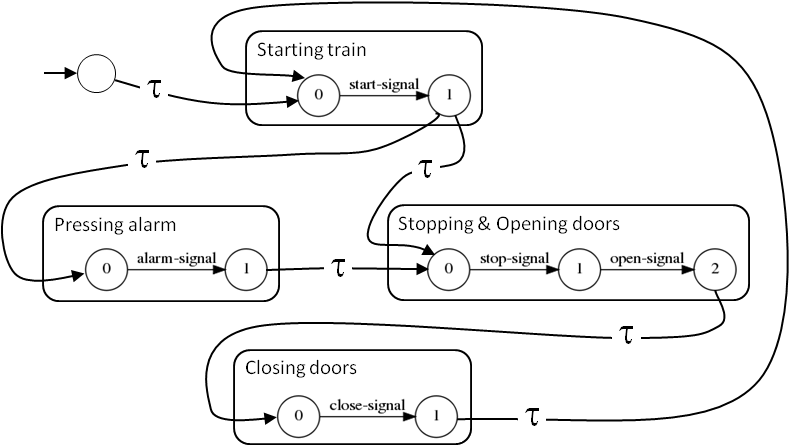
\includegraphics[trim=0mm 0mm 0mm 0mm, clip]{src/2-framework/images/train-controller-synthesis}
}
\caption{Synthesis of the \emph{Controller} LTS from the hMSC of Fig.~\ref{image:train-hmsc}.\label{image:train-controller-synthesis}}
\end{figure}

An important difference should be noted between the relations between MSC languages in equation (\ref{equation:msc-composition}) and those on hMSC languages in (\ref{equation:hsmc-traces-by-agent-composition}). The former denotes an equality between $\mathcal{L}_{partial}(M)$ and $\mathcal{L}(M_{\downarrow Ag_1}\parallel\ldots\parallel M_{\downarrow Ag_n})$ whereas the latter defines a set inclusion between $\mathcal{L}_{weak}(H)$ and $\mathcal{L}(H_{\downarrow Ag_1}\parallel\ldots\parallel H_{\downarrow Ag_n})$. In fact, traces in $\mathcal{L}_{arch}(H) \setminus \mathcal{L}_{weak}(H)$ capture the set of \emph{implied} scenarios of a hMSC specification~\cite{Alur:2000, Uchitel:2004}. Implied scenarios occur when a system is designed globally while implemented component-wise. In other words, implied scenarios capture traces that follow different paths in the hMSC when projected on individual agent timelines. Implied scenarios are further discussed in Section~\ref{section:background-discussion}.

\subsection*{hMSCs composed from finer-grained hMSCs}

As stated previously, a hMSC node may refer to a finer-grained hMSC instead of a bMSC. To take the latter into account in the trace semantics given previously, we must decide how a sub-hMSC is to be ``connected'' with its father. To keep a consistent framework in terms of synchronization hypotheses, we require such sub-hMSC to have, in addition to its initial state, a terminating state to which at least one node is connected. For simplicity, we also forbid nodes with no outgoing transition. 

Under those assumptions, it is relatively easy to unfold a compound hMSC into another one where all refined nodes are basic MSCs. The trace semantics remains unchanged and is defined in terms of the latter ``flat'' hMSC. 

In practice, this flat hMSC must not be explicitly constructed when the LTS for $\mathcal{L}_{arch}$ is synthesized. The LTSs $H_{\downarrow Ag_i}$ for finer-grained hMSCs meeting our constraints have only one initial state and only one terminating state; this allows them to be connected with $\tau$ transitions in the same way as the LTSs $M_{\downarrow Ag_i}$. A similar argument applies for $\mathcal{L}_{strong}$.

\subsection{Explicit state annotations\label{subsection:background-scenario-annotations}}

MSCs are often annotated with state-based information (see, e.g.,~\cite{VanLamsweerde:1998, Kruger:2000, Whittle:2000}). 

TODO: complete this description, discussing the difference between identification and state assertions (aka fluent-based decorations). The former info uniquely identifies an agent state, so that they can be merged with mandatory merge constraints presented in section~\ref{section:inductive-from-hMSC}, while the later does not, but helps pruning search space as usual with fluents.

\subsection{Consistency between the scenario and agent behaviors views\label{subsection:background-scenario-consistency}}

The trace semantics of scenarios can be explicitly related to agent and system behaviors as the latter are captured with LTS (see Section~\ref{section:background-state-machines}). This section defines consistency rules between those two views, and explains the similarity between equations (\ref{equation:system-composition}), (\ref{equation:msc-composition}) and (\ref{equation:hsmc-traces-by-agent-composition})

\subsubsection*{Positive and negative MSCs}

Consider a system composed of $n$ agents whose behavior is modeled by $\system$. Let $M$ denote a MSC illustrating interactions among them. $M$ and $S$ are said to be \emph{consistent} if the following conditions hold:

\begin{itemize}
\item $M$ and $S$ are \emph{strucurally} consistent,
\item $\mathcal{L}(M_{\downarrow Ag_i}) \subseteq \mathcal{L}(Ag_i)$ for each agent $Ag_i$
\item $\mathcal{L}(M) \subseteq \mathcal{L}(S)$
\end{itemize}

\noindent where, for recall, $\mathcal{L}(M) = \mathcal{L}(M_{\downarrow Ag_1} \parallel \ldots \parallel M_{\downarrow Ag_n})$

The first condition requires the MSC and the system to agree on the set of agents and their respective interfaces. A MSC may actually illustrate interactions among a proper subset of system agents. However, labels along a timeline must be a subset of the alphabet of the corresponding agent. The second condition states that the traces defined by a timeline in the MSC must be traces accepted in the LTS modeling the behavior of the corresponding agent.  The third condition states that all linearizations of the MSC must be accepted traces in the LTS modeling the behavior of the composed system. Note that, under structural consistency, the second condition implies the third one~\cite{Uchitel:2003}.

Similarly to positive MSCs, a negative MSC $N = (P,e)$ and a system $\system$ are said to be consistent if the following condition hold:

\begin{itemize}
\item $N$ and $S$ are \emph{strucurally} consistent,
\item $P$ and $S$ are consistent, and
\item $\mathcal{L}^{-}(N) \not\subseteq \mathcal{L}(S)$
\end{itemize}

The first condition is similar to what has been said previously for positive MSCs. The second enforces the precondition to be a consistent positive MSC; it implicitly requires positive traces to be accepted. The last condition states that the system may not exhibit any negative trace captured by the negative MSC.

\subsubsection*{Scenario collections}

A scenario collection $Sc = (S^+,S^-)$ and a system are said to be consistent if and only if each positive and each negative MSC of the collection is itself consistent with the system. 

Moreover, a set $S^+$ of positive scenarios and a set $S^-$ of negative scenarios are consistent with each other if there exists a system which is consistent with them taken as a collection $Sc = (S^+,S^-)$. 

A necessary condition for a scenario collection to be consistent is the disjointness of positive and negative traces:

\begin{center}
$Sc = (S^+,S^-)$ is consistent only if $\mathcal{L}^+(Sc) \cap \mathcal{L}^-(Sc) = \emptyset$
\end{center}

This condition is not sufficient however because structural consistency is not taken into account.

By definition, a collection cannot be consistent with a system unless all scenarios start in its initial state. This may imply a lot of redundancy in the description of large systems. Consistency might be difficult to guarantee without costly refactoring on scenarios. Also, since scenarios and scenario collections are both finite, a collection is rarely complete in practice; most systems accept an infinite number of traces, through loops.  High-level Message Sequence Charts (hMSCs), introduced in the next section, provide a means for tackling these problems.

\subsubsection*{High-level MSCs}

A hMSC $H$ and a system $\system$ are said to be consistent if the following condition holds:

\begin{itemize}
\item $H$ and $S$ are \emph{structurally} consistent,
\item $\mathcal{L}(H_{\downarrow Ag_i}) \subseteq \mathcal{L}(Ag_i)$ for each agent $Ag_i$,
\item $\mathcal{L}_{arch}(H) \subseteq \mathcal{L}(S)$
\end{itemize}

\noindent where, for recall, $\mathcal{L}_{arch}(H) = \mathcal{L}(H_{\downarrow Ag_1} \parallel \ldots \parallel H_{\downarrow Ag_n})$

These conditions are the counterpart of those given previously for MSCs. They have a similar interpretation, \emph{mutatis mutandis}. 

Moreover it is convenient to distinguish between a hMSC that describes all behaviors of a system and one that only illustrates a subset of them. This leads to the notion of hMSC completeness. 

A hMSC $H$ is \emph{complete} for a system $\system$ if it is consistent with it and defines the same language, that is, if the following condition holds

\begin{equation}
\mathcal{L}_{arch}(H) = \mathcal{L}(S)
\end{equation}

